\section{Analysis}
\label{sec:Auswertung}
The following calculations are made with  "Numpy" \cite{numpy}, 
"Uncertainties" \cite{uncertainties}, 
"Scipy" \cite{scipy} and  "Matplotlib" \cite{matplotlib}.

%%%%%%%%%%%%%%%%%%%%%%%%%%%%%%%%%%%%%%%%%%%%%%%%%%%%%%%%%%%%%%%%%%%%%%%%%%%%%%%%%%%%%%%%%%%%%%%%%%%%%%%%%%%%
\subsection{Fitting the linear expansion coefficient}
For the following calculations the expansion coefficient is needed.
For that purpose the data in table \ref{tab:alpha}
is fittet with
\begin{equation}
    \alpha = a \frac{1}{T} + b:
    \label{eq:alpha}
\end{equation}
\begin{equation*}
    a = -873 \pm 4
\end{equation*}
\begin{equation*}
    b= 19.411 \pm 0.029
\end{equation*}

\begin{figure}
    \centering 
    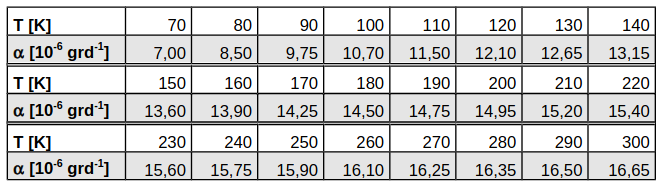
\includegraphics[width=\textwidth]{build/alpha.pdf}
    \caption{The expansion coefficient plottet against the temperature and the corresponding fit.}
\end{figure}

%%%%%%%%%%%%%%%%%%%%%%%%%%%%%%%%%%%%%%%%%%%%%%%%%%%%%%%%%%%%%%%%%%%%%%%%%%%%%%%%%%%%%%%%%%%
\subsection{Calculating the molar heat capacity}
For the calculation of the molar heat capacity 
the current $I$, voltage $U$ , time $t$ and resistance $R$ are measured 
like described in section \ref{sec:Durchführung} (see Table \ref{tab:Messwerte}).
\newline \newline
\noindent The engergy the coppy receives is calculated by 
\begin{equation}
    E = U \cdot I \cdot \Delta t .
\end{equation}
\noindent With \eqref{eq:T} and the resistance $R$ the temperature $T$ is determined.
The molar heat capacity for constant pressure ist calculated by
\begin{equation}
    c_p = \frac{ M}{m} \frac{E}{\Delta T}.
\end{equation}
\noindent $M = \SI{63.55}{\g\per\mole}$ is the molar Mass and
$m= \SI{342}{\g}$ \cite{Molmasse_kupfer}\cite{V47}.
The molar heat capacity for constant volume is calculated with 
\begin{equation}
    c_v = c_p - 9 \alpha^2 \kappa V_0 \cdot T.
\end{equation}
\noindent $\kappa = 140 \si{\N\per\square\m}$ is the compression modulus \cite{kappa_kupfer}
and $V_0 = V_0 =  7.11 \si{\cubic\cm\per\mole} $ is the molar Volume \cite{V0_kupfer}.
The results are plottet in figure \ref{fig:cv} and listet in table \ref{tab:cv}.

\begin{figure}
    \centering 
    \includegraphics[width=\textwidth]{build/c_v.pdf}
    \caption{The heat capacity for constant volume $c_v$ plottet against the temperature $T$.}
    \label{fig:cv}
\end{figure}

%%%%%%%%%%%%%%%%%%%%%%%%%%5
\subsection{Determining the Debye temperature}
\label{sub:deb}
\subsubsection{Empirically}
With $c_v$ and the table \ref{tab:deb}
$\frac{\Theta_D}{T}$ and $\Theta_D$ can be determined (see table \ref{tab:deb2}).
Then the mean and standard deviation is calculated:
\begin{equation*}
    \bar{\Theta}_D =  (460 \pm 100) \si{\kelvin}
\end{equation*}

\begin{table}
    \centering
    \sisetup{table-format = 1.2}
    \begin{tabular}{c c c c}
        \toprule
        $T$ in $\si{\kelvin}$ & $c_v$ in $\si{\joule\per\mole\per\kelvin}$ & $\frac{\Theta_D}{T}$ & $\Theta$ in $\si{\kelvin}$ \\
        \midrule
        103,3  &  16,78  &  4,6  &  475,2  \\
        113,3  &  17,38  &  4,7  &  532,6  \\
        123,4  &  18,50  &  4,9  &  604,6  \\
        133,3  &  19,22  &  3,5  &  466,4  \\
        143,2  &  19,86  &  3,6  &  515,5  \\
        153,1  &  20,36  &  2,0  &  306,3  \\
        163,2  &  21,29  &  2,1  &  342,6  \\
        \bottomrule
    \end{tabular}
    \caption{$c_v$,$\frac{\Theta_D}{T}$ and $\Theta_D$ for $T < 170 \si{\kelvin}$. }
    \label{tab:deb2}
\end{table}

\subsubsection{Theoretically}
The Debye temperature $\Theta_D$ can be calculated with \eqref{eq:omega}.
$N_L$ and $L^3$ are replaced with
\begin{equation*}
    N_L = \frac{N_A \cdot m }{M} \quad \text{and} \quad L^3= \frac{m}{\rho},
\end{equation*}
so that $\Theta_D$ can also be calculated with
\begin{equation}
    \Theta_D = \frac{\hbar}{k_B} \left( \frac{18 \pi^2 N_A \rho}{M}\left( v^{-3}_l + 2 v^{-3}_t\right)\right)^{\frac{1}{3}} = 332.0 \si{\kelvin}
\end{equation}
\noindent for $\rho = 8.92 \si{\kg\per\cubic\cm}$ \cite{V0_kupfer},
 $v_l=4.7 \si{\km\per\s}$ and $v_t=2.26 \si{\km\per\s}$ \cite{V47}.

